\section{Klassen, Features und Selektoren}
    \label{section:conceptClassesFeaturesSelectors}
    Mit dem \gls{wccs} sollen Inhalte klassifiziert,
    das heißt einer von vielen Klassen zugewiesen werden.
    Dieses Kapitel erläutert, was eine Klasse im Kontext des \glspl{wccs} ist
    und mit welchen anderen Konzepten es in Beziehung steht.

    \subsection{Klassen}
        Der Begriff "`Klasse"' stammt aus der Mathematik und beschreibt eine Menge von Objekten,
        die eine gemeinsame Aussage erfüllen \cite{oberschelp:Mengenlehre}.
        Eine Klasse kann deshalb eindeutig gebildet werden.
        Diese Definition erfährt für das \gls{wccs} eine Erweiterung,
        die in Abbildung \ref{image:conceptClasses} modelliert wird.

        \begin{figure}[htb]
            \centering
            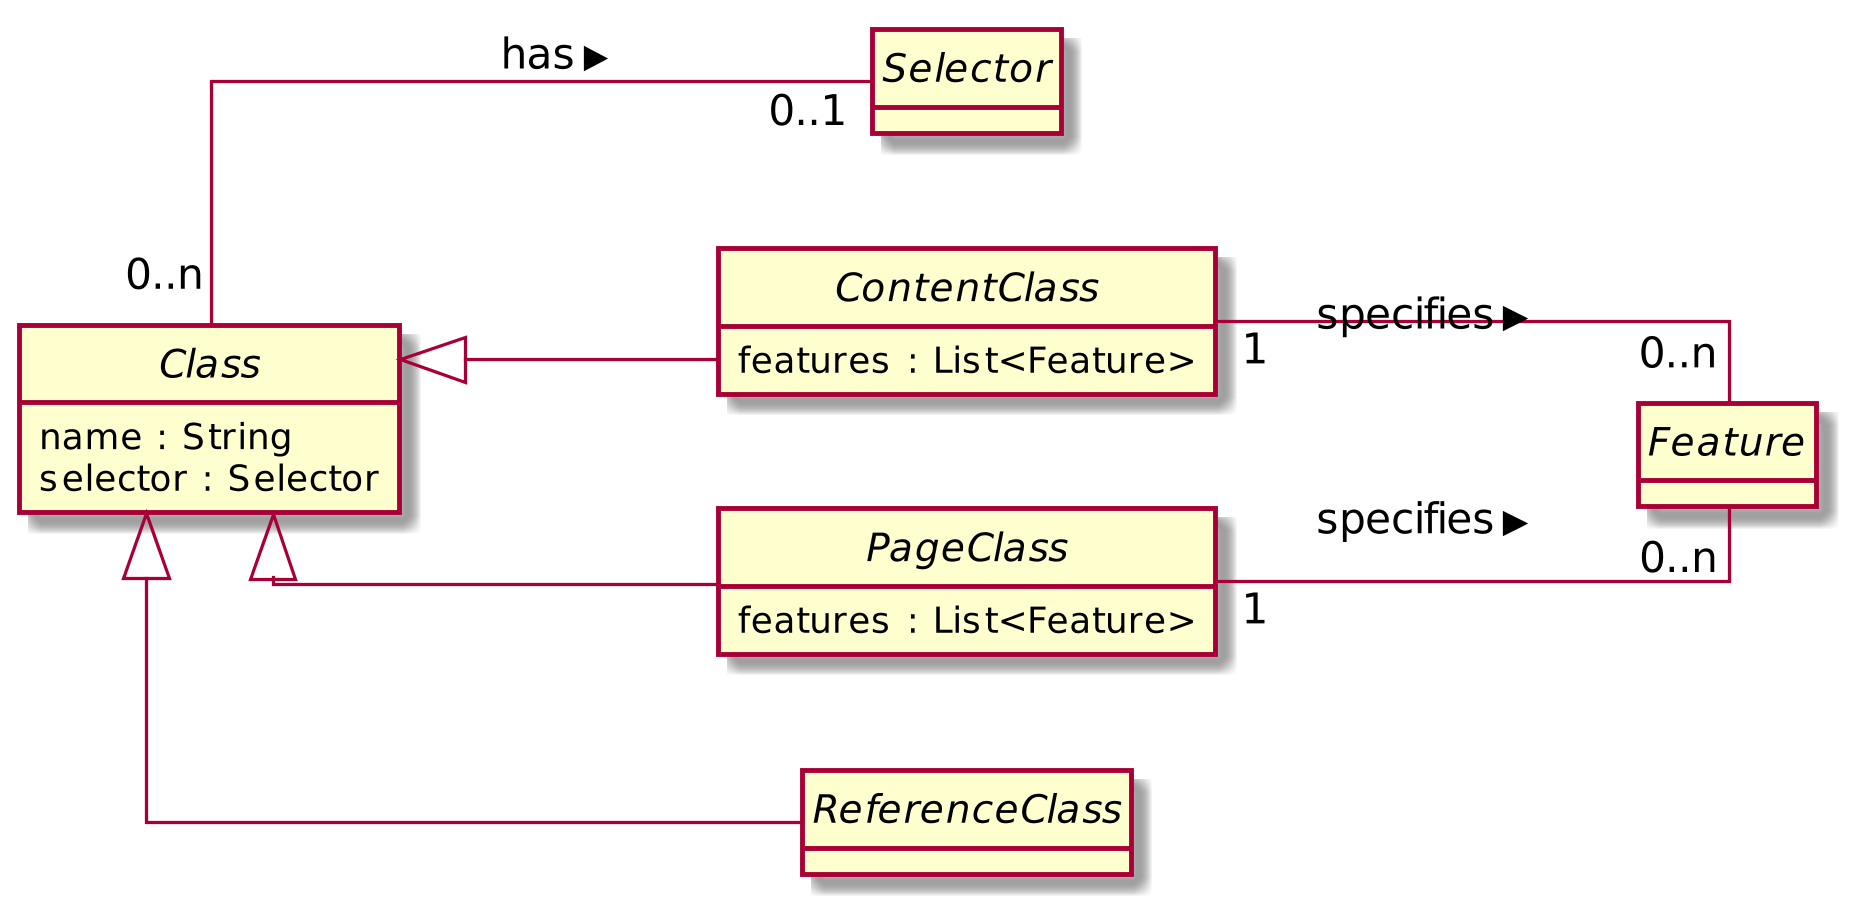
\includegraphics[width=\textwidth]{../resources/concept/classes.png}
            \caption{Klassen im Kontext des \acrshortpl{wccs}}
            \label{image:conceptClasses}
        \end{figure}

        Die zu klassifizierenden Entitäten sind Seiten, Inhalte und
        Referenzen\footnote{vgl. Kapitel \ref{section:classificationEntities}},
        weshalb das System drei Arten von Klassen kennt:

        \begin{enumerate}
            \item Seitenklassen,
            \item Inhaltsklassen und
            \item Referenzklassen.
        \end{enumerate}

        Jeder Klasse ist gemein, dass sie einen Namen und einen bis zu einen Selektor hat.
        Selektoren stellen Aussage dar, die Elemente einer Klasse erfüllen müssen,
        wie in mathematischer Definition erklärt.
        Auf Selektoren wird weiter in Kapitel \ref{section:conteptSelectors} eingegangen.
        Seiten und Inhaltsklassen spezifizieren außerdem beliebig viele Bestandteile
        (im weiteren Verlauf Features genannt).
        Referenzklassen tun dies nicht, weil das \gls{wccs} nicht vorsieht, dass eine Referenz eine komplexe hierarchische Struktur hat.
        Werden im folgenden Kapitel \ref{section:conceptFeatures} erläutert.
        Klassen werden einmalig definiert und können anschließend zur Klassifikation beliebig vieler Seiten herangezogen werden.
        Oder für beliebige Features. Siehe nächstes Kapitel.

    \subsection{Features}
        \label{section:conceptFeatures}
        Wie in Kapitel \ref{section:requirements} beschrieben, besitzt eine Seite eine
        hierarchische inhaltliche Struktur, die durch die Klassifikation abgebildet werden muss.

        Dazu führt das \gls{wccs} das Konzept der Features ein.
        Features sind wie oben erwähnt Teil einer Seiten- oder Inhaltsklasse
        mit denen die Struktur eines klassifizierten Elementes beschrieben wird.
        Eine Feature besitzt deshalb auch eine Klasse.
        Nachdem Objekt in eine Klasse eingeordnet wurde,
        wird versucht Teile des Objektes gemäß den Features der Klasse weiter zu klassifizieren.
        Ein Objekt besitzt also eine Klasse und seine Teile können spezifischer klassifiziert werden.
        Da Klasse eines Features selbst auch Features besitzt, entsteht also eine hierarchische Klassifikation.
        Damit kann die Struktur einer Seite abgebildet werden.

        Beim Beispiel aus Kapitel \ref{section:requirements} hieße das:
        Seite wird mit Seitenklasse "`Service"' klassifiziert.
        Diese Klasse hat ein Feature "`faqThema"' welches als "`FaqSection"'
        klassifiziert wird.
        Diese Klasse hat ein Feature "`faqEintrag"' mit der Klasse "`FaqEntry"'.
        Diese hat wiederum die Features "`question"' und "`answer"' mit den Klassen
        "`FaqQuestion"' und "`FaqAnswer"'.
        % TODO: Vielleicht ist das hier nicht notwendig, falls Beispiel-Transformation schon in Kapitel 1/2 erfolgt.

        Dieser Zusammenhang und noch mehr wird in Abbildung \ref{image:conceptFeatures} modelliert.

        \begin{figure}[htb]
            \centering
            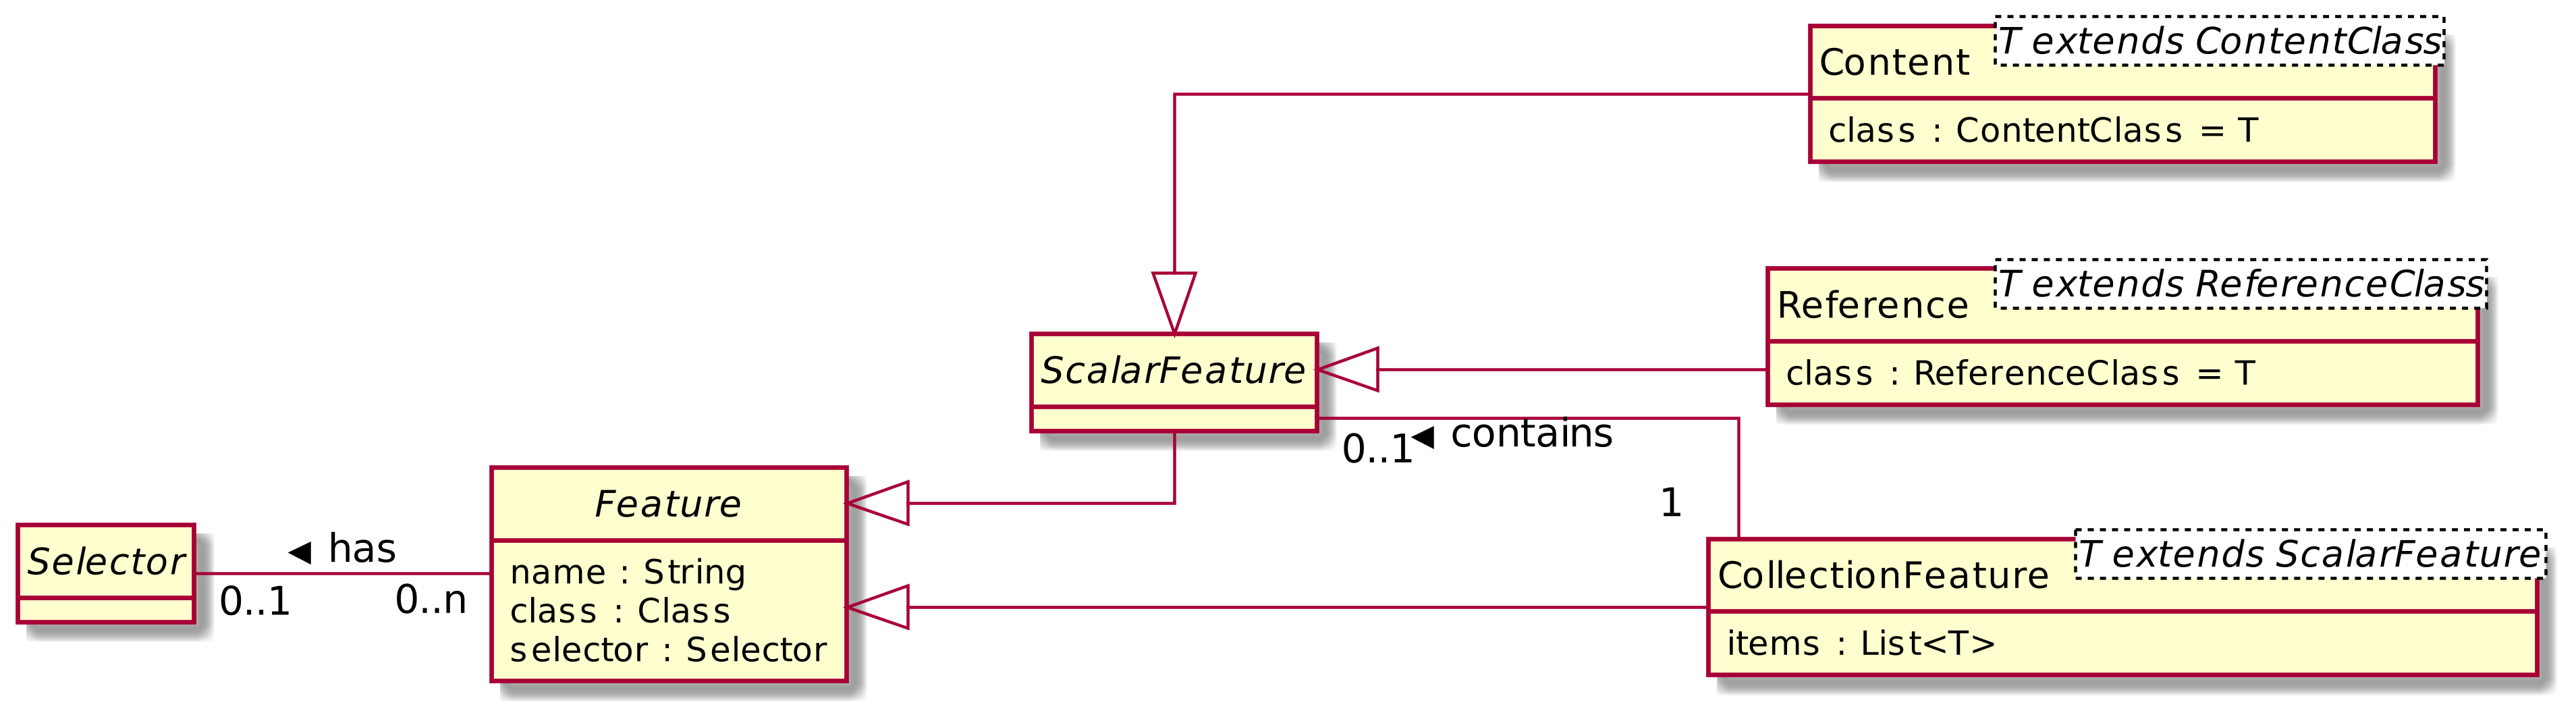
\includegraphics[width=\textwidth]{../resources/concept/features.png}
            \caption{Features}
            \label{image:conceptFeatures}
        \end{figure}

        % TODO Parent und Child Feature

        Es gibt zwei konkrete Arten von Features: Inhalt (Content Feature) und Referenz (Reference Feature).
        Jedes Feature hat einen Namen und eine Klasse.
        Content Features klassifizieren Inhalt, weshalb die Klasse auch eine Inhaltsklasse sein muss.
        Entsprechend muss die Klasse einer Referenz auch eine Referenzklasse sein.
        Features können darüber hinaus bis zu einem Selektor besitzen.
        Wieso berschreibt Kapitel \ref{section:conteptSelectors}.
    
        Neben dem was Features klassifizieren, lassen sich Features auch noch nach der
        Kardinalität einer konkreten Klassifikation unterteilen.
        Zunächst gibt es einelementige Features.
        D.h. ein Feature enthält genau eine Klassifikation.
        Wird deshalb ScalarFeature bezeichnet.
        Auf der anderen Seite kann ein Feature auch eine Menge von Klassifikationen
        darstellen, für den Fall, dass viele Elemente mit einer Eigenschaft gefunden wurden
        und alle unter einem Namen zusammengefasst werden sollen.
        Eine solches CollectionFeature enthält eine Menge von konkreten ScalarFeatures,
        wobei jedes Feature dieselbe Content- bzw. ReferenceClass verwendet.
        Das wird im Modell dadurch angezeigt, dass Content- und ReferenceClass teil der Typdefinition
        von Content- und ReferenceFeature sind.
        Jedes Element in einem CollectionFeature kann seine eigene Struktur haben.
        Prinzipiell wäre es auch möglich Features immer als Liste darzustellen
        und anstelle von ScalarFeatures eine einelementige Liste zu haben.
        Die Handhabung eines Objektes ist aber leichter in diesem Fall und außerdem drückt
        die Unterscheidung die Intention des Features besser aus.
        Einelementige Liste oder viele Treffer für skalares Feature können auf Fehler in der
        Klassendefinition hinweisen.

        Durch Features werden konkrete Inhalte oder Referenzen auf einer Seite klassifiziert.
        Wie später noch genauer erklärt wird:
        Ein Feature klassifiziert dabei genau ein HTML-Element auf der Seite.
        Jedes Element in einem CollectionFeature klassifiziert genau einen HTML-Node.
        Child Features klassifizieren entsprechend HTML-Child-Nodes.
        Eine Konsequenz ist, dass Text innerhalb eines Nodes nicht einzeln selektiert werden kann.
        % TODO: WARUM HAT MAN SICH DAFÜR ENTSCHIEDEN?

    \subsection{Selektoren}
        \label{section:conteptSelectors}
        Die bisher beschriebenen Klassen und Features beschreiben nur
        die erwartete Struktur einer Seite und wie die jeweiligen Elemente klassifiziert
        werden sollen.
        Bisher nicht darauf eingeangen, anhand welcher Aussagen das \gls{wccs} Objekte
        in Klassen einteilt.
        Diese Aufgabe übernehmen Selektoren für die es zwei Anwendungsfälle gibt:
        Klasse einer Seiten (Seitenklasse) bestimmen.
        Dafür definiert jede Seitenklasse zwingend einen Selektor.
        Dieser Selektor kann auf eine gegebene Seite angewandt und entschieden werden,
        ob Seite zur Klasse gehört.
        Zweiter Fall ist Feature in einem klassifizierten Element ausfindig machen.
        Erste Möglichkeit ist Selektor zu verwenden, der über Klasse des Features definiert wird.
        Allerdings auch sinnvoll diesen Selektor bei Bedarf für ein einzelnes Feature zu überschreiben,
        um Unregelmäßigkeiten auf den Seiten zu kompensieren.
        Deshalb kann Selektor auch am Feature definiert werden.
        Wichtig ist, dass Selektor für ein Feature ableitbar ist.
        Deshalb ist es ausreichend, wenn er am Feature oder an der Klasse definiert ist.
        Content- und ReferenceKlassen brauchen deshalb nicht zwingend einen Selektor.

        Welche Arten von Selektoren das \gls{wccs} konkret unterstützt,
        wird in Kapitel \ref{section:conceptClassification} erklärt.